%===========================================================
%                              Choix de thématique
%===========================================================
% Une des quatre options 'parallelisme', 'architecture', 'systeme' 
% 'tempsreel' doit être utilisée avec le style compas2021
\documentclass[systeme]{compas2022}
\usepackage{algorithm2e}

%===========================================================
%                               Title
%===========================================================

\toappear{1} % Conserver cette ligne pour la version finale

\begin{document}

\title{Correct and high performance database}
\shorttitle{TCC}

\author{Saalik Hatia}%

\address{Université Pierre et Marie Curie\\
Laboratoire LIP6 \\
4, place jussieu\\
75005 Paris - France\\
saalik.hatia@lip6.fr}

\date{\today}

\maketitle

%===========================================================         %
%R\'esum\'e
%===========================================================  
\begin{abstract}
  Le fichier fonctionne en \LaTeXe. La taille
  de ce résumé peut atteindre une dizaine de lignes.
  \MotsCles{un maximum de 5 mots significatifs, en français, doivent être 
    isolés sous forme de mots-clés.}
\end{abstract}

\tableofcontents

%=========================================================
\section{Introduction}
%=========================================================

Modern planet-scale applications increasingly use distributed database system to provide users with fast, available and consistent data.
But existing database are built without any formalising in mind.
They have bugs that impact the consistency and integrity of their data.
We aim to build a database that is correct by design and performant.
Formalising a database that provide users with fast read and writes, data safety and geo replication is hard.
Instead of trying to formalize a database with all these features we propose the following approach.
We decompose the database we are aiming for into simpler, smaller models.
We adopt a stepwise approach starting with a bare-bones and obviously correct concurrent database system, then at each step we add features, like persistency, caching, checkpointing and geo-distribution. 
Each step adds a single feature.
For every step we describe its key invariants, formalize an operationnal semantics, and provide a reference implementation.
Then we compare the different models between them and show through testing that the implementations are equivalent.
Ultimately, we show that our final design is both correct and is equivalent to other equivalent databases in terms of perfomance.
We claim to provide developers with a clear model that allows them to implement a correct, high performance and geo-distributed database.


%=========================================================
\section{Interface and transactions}
%=========================================================

We define two main actors in our system:
\begin{itemize}
  \item A client: interacts with the database using Application Programming Interfaces (APIs) exposed by the database
  \item Database: hosts data that is read and written by the client.\\
\end{itemize}

In this paper a client only interacts with the database through transactions, which are a sequence of read and write operations.
The API is the following:
\begin{itemize}
  \item \emph{begin(Dt)} initializes a transaction with a snapshot
  \item \emph{read(key): blob} returns the object \emph{key} from the snapshot
  \item \emph{effect(key,blob)} assigns a the value \emph{blob} to the key \emph{key}
  \item \emph{abort()} abort the live transaction
  \item \emph{commit()} attempts to commit, if it succeds assigns a commit timestamp to the transaction; otherwise the transaction aborts.
\end{itemize}


%=========================================================
\subsection{Transactions}
%=========================================================

A transaction is a sequence of read and write operations followed by a commit or an abort.
An operation is either a read or a write from the transaction's snapshot called \emph{Dependency Snapshot}.
And the visibility of these operations are atomic at the time of commit.

There are three main phases in the lifecycle of a transaction.
A transaction starts with a begin phase where the transaction is initialized, in the operational phase the client executes operations and finally termination that ends the transaction.
During these phases a transaction goes through two state, \emph{live} and \emph{terminated}.

A transaction is represented using the following information:
\begin{itemize}
\item \emph{$\tau_i$} Unique transaction identifier.
\item \emph{Dt} Dependency timestamp which represent a snapshot the transaction will interact with.
\item \emph{$\varepsilon$} Effect map contains the writes made by the transactions.
\item \emph{R} Read set which records the keys of objects read by the transaction.
\item \emph{Ct} a commit timestamp that represent the time at which the timestamp has been committed.
\item \emph{State} the state of the transaction is either \emph{live} or \emph{terminated}.\\
\end{itemize}

During the begin phase a transaction is assigned a unique identifier $\tau_i$ and a \emph{Dependency Snapshot Timestamp} ($Dt$), while the Effect Map, Read Set and the commit timestamp are initialized to \emph{null}. Finally the state of the transaction is set to \emph{live}.

During the operation phase any number of operations are executed.
A Read updates the Read Set $R_i$ and a write updates the Effect Map $\varepsilon_i$.

In termination phase the transaction either commits or aborts depending on client and system invariants. 
The transaction's state is then set to \emph{terminated}

\subsection{Timestamps and snapshots}

We use timestamps as method of concurrency control.
Every transaction has a timestamp (Ct) that is assigned by the system when the transaction is committed.
It is used to perform arbitration on the order of the transactions.

Using these timestamps we define a snapshot as a collection of transaction that have a commit timestamp less than or equal to a timestamp.
The latter is called the Dependency Snapshot Timestamp.

Snapshots provide \emph{isolation} guarantees to the system, meaning a client only reads object versions that are part of the snapshot and are committed. 
In addition to isolation, snapshots also provide the client with \emph{atomicity} guarantees: $\varepsilon_i$ of a transaction $\tau_i$ are seen in an all-or-nothing manner.

\subsection{Object-version}

Having only one version of an object severly limits concurrency in a database.
Multi-Version Concurrency Control (MVCC) is a technique that allows a database to have multiple versions of an object (Object-Versions).
Every update to an object creates its own version and to ensure that all transactions read the correct version of an object the system maintains the following information: 
\begin{itemize}
  \item \emph{key} is the unique identifier of the object.
  \item \emph{$\tau_i$} identifier of the transaction that wrote this version.
  \item \emph{blob} is a pointer to the value of the materialized object.
\end{itemize}

In this paper we note object-version by $(key ,\tau_i)$.

\section{System Model}

Starting from a simple in memory Key-Value store, we describe the model then progressively add features and compare every progression between them (\emph{figure \ref{fig:transitions}}).
We provide an implementation for every model and compare implementations between them to show that the implementation are equivalent.

\begin{figure}[tp]
  \centering
  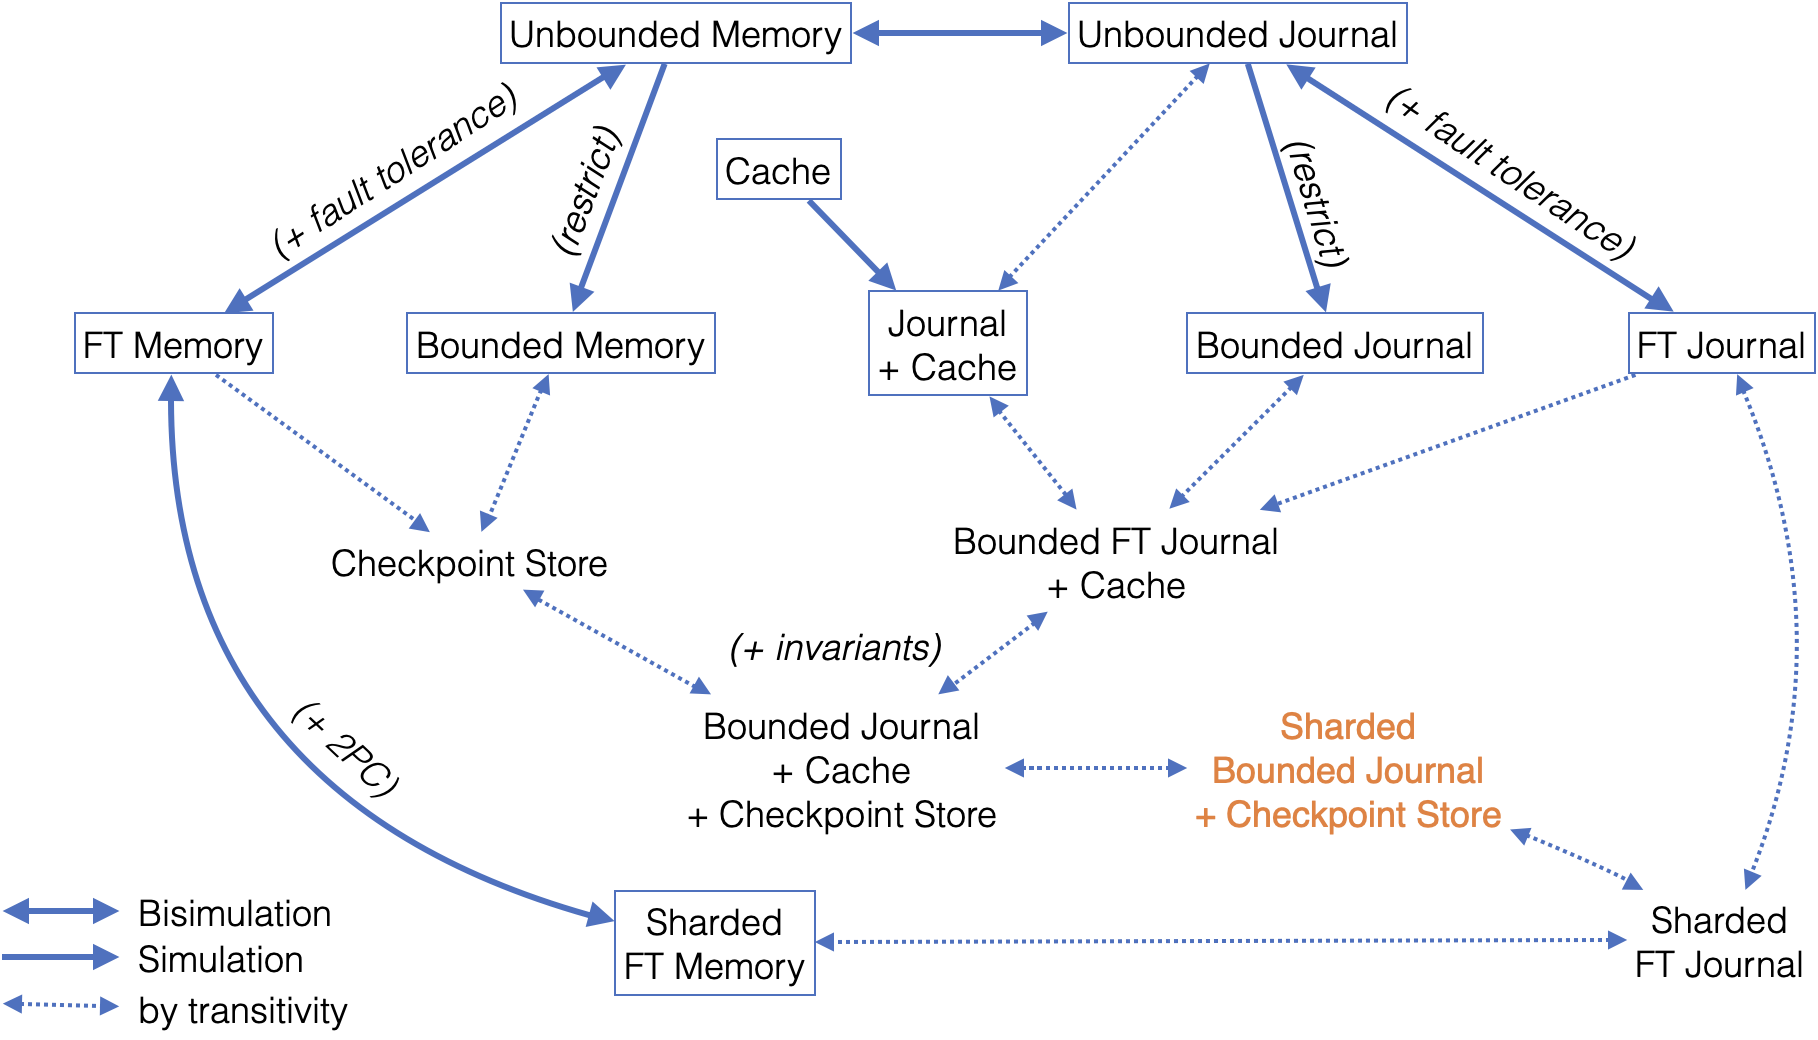
\includegraphics[width=0.75\textwidth]{figures/transitions.png}
  \caption{Progressions in our model}
  \label{fig:transitions}
\end{figure}

\subsection{Transactional Causal Consistency (TCC)}

Our model supports multiple consistency levels. In this work however, we focus on Transactional Causal Consistency (TCC).
TCC means that: (1) if one update happens before another, they will be observed in the same order (causal consistency), and (2) updates in the same transaction are observed all-or-nothing.

To keep track of happened-before, we use timestamp to order updates.
When a transaction $\tau_i$ commits, it is assigned a commit timestamp $Ct_i$ timestamp and the effects $\varepsilon_i$ moved into the store with as object versions $(key,Ct_i)$.
These occur atomicallu with regard to any other transactions.
If a transaction $\tau_j$ has a dependency $Dt_j$ higher than $Ct_i$ than all the effects of $\tau_i$ are visible for $\tau_j$.

Reformuler en expliquant pourquoi les CRDT ici(Conflits are taken care of by using CRDTs as our data type ensuring that reading from a snapshot $St$ is determistic.)

We introduce our first system invariant:

\[
  \begin{array}{lcl}
    \emph{$Dt_i < Ct_i$}
  \end{array} 
\]

\subsection{Unbounded Memory}

We start with a simple in-memory key-value store.
All the database is stored in volatile memory therefore if a crash or restart occurs the database is lost.

The Unbounded Memory model stores Object-version $key_{\tau_id}$ in memory.
In adition to the object version the transaction information are also stored in memory in order to track information necessary to uphold our consistency guarantees.

Because this model is memory only, all data is lost is a crash or a restart happens.
Therefore there are no invariants regarding persistency or recovery.
Additionally we consider the memory to be unbounded so there are no restriction on the size of the data or constraints on the dependency timestamps.

\subsection{Transaction invariants}

For every transaction we define the following invariants.
In order to ensure that every operation is done within a transaction our model require that each API call except \emph{begin()} checks if there is a $live$ transaction for the calling client.

When a transaction commit it is causally dependent on the Snapshot reprensented by $Dt$.
We represent this by assigning a commit timestamp $Ct_i$ higher than the dependency timestamp.

These are the transaction invariants maintained during transactions:
\[
  \begin{array}{lcl}
    \emph{$Dt_i < Ct_i$}\\
    \emph{$(read, effect, commit, abort) => State = live$}
  \end{array} 
\]


TODO Le premier invariant est un peu faible tout seul. Il faut ajouter le fait qu'il est valable pour toutes transactions committées. Les sections suivantes sont sous forme de texte mais elle seront mise sous forme de pseudo code avec les precondition et les invariants.\\


\textbf{Start transaction}
When a client starts a transaction, if the client specify a dependency timestamp $Dt$ the system checks if it is valid in regards to consistency guarantees and creates a transaction object.
If no dependency timestamp is specified than the transaction is initialized with a valid dependency timestamp.
The transaction is then assigned a unique transaction identifier $\tau_i$ and $\emph{State} \leftarrow \emph{live}$ \\

Postconditions:\\
$State_i \leftarrow \emph{live}$ \\


\textbf{Read}\\
Preconditions:\\ 
$State_i = \emph{live}$ \\

Returns the Object-version k from the snapshot \emph{Dt}. 
If the object doesn't exist the system returns a default value.

In case a transaction attempts to read an object that has concurrent updates, we use CRDTs in order to ensure that the merge is determistic.
The system adds the key to the read set of the live transaction.\\
$R_i \leftarrow \emph{key}$\\

\textbf{Effect}\\
Preconditions:\\ 
$State_i = \emph{live}$ \\

Applies the effect on the object present in the snapshot \emph{dt} resulting in the creation of a new object-version.
The object version is then added to the Effect Map of the live transaction.\\
$\varepsilon \leftarrow key_{\tau}$

\textbf{Commit transaction}\\
Preconditions:\\ 
$State_i = \emph{live}$ \\

When a transaction is committed the system checks if the transaction is valid in regard to the consistency model chosen by the system.
If everything is correct then the transaction is committed and the transaction is assigned a commit timestamp such as $Dt_i \leq Ct_i$.

All the effects of the transaction are then available for transaction that have $Dt_j \geq Ct_i$.\\

Postconditions:\\
$State_i \leftarrow \emph{terminated}$ \\
$Dt_i \geq Ct_i$.\\



\textbf{Abort transaction}
Preconditions:\\ 
$\emph{State} = \emph{live}$ \\

If a transaction is aborted then all the effects of the transaction are void.

Postconditions:\\
$State_i \leftarrow \emph{terminated}$ \\

\subsection{Bounded Memory}

In the Bounded Memory model we choose to define an arbitrary limitation on the size of the memory used by the system.

\textbf{System invariants}
All system invariants from the Unbounded memory are present here.
Plus we introduce a two new value:
\begin{itemize}
  \item \emph{$M_{used}$} contains the current size of data in memory
  \item \emph{$M_{limit}$} represents the maximum size available to the database
\end{itemize}
Based on these two variable we introduce a new system invariant:
\begin{itemize}
  \item \emph{$M_{used}$} $<$ \emph{$M_{limit}$}
\end{itemize}
In order to uphold the memory constraints of the system we keep track of all the dependencies of running transactions called \emph{RunningTr} but also all the commit timestamps of finished transactions \emph{CommitTr}.

We then introduce a new timestamp called Minimum Dependency \emph{MinDt}.
\emph{MinDt} represents the oldest snapshot any running transaction is reading from.
When a transaction $\tau_i$ commits or aborts, it is removed from \emph{RunningTr}. 
And if $Dt_i = MinDt$ and no other transaction is reading from $Dt_i$ the system advances \emph{MinDt} to the next oldest snapshot used in \emph{RunningTr}.



\subsection{Garbage collectio - WIP}
When \emph{$M_{used}$} $\geq$ \emph{$M_{limit}$}. 
All the transaction in the system are halted in order to perform a garbage collection.

Ici je dois expliquer comment est fait le GC:\\
\begin{algorithm}
  \KwIn{\\ \Indp
    RunningTr : set
  }
  \(oldTr \longleftarrow \emptyset\)\;
  \ForAll{\(\tau_{i} \in Running\)}{
    \If{\(Dt_{i} < MinDt\)}{
      \(oldTr \longleftarrow \tau_i\)\;
    }
  }
\end{algorithm}

WIP


\subsection{Implementation - WIP}

Every model is implemented in java with external libraries for persistency, CRDTs and data structures that we consider being correct.
Implementation and evaluation of the different models have two purposes.
First we implement our different models as closely as possible to our specification and show that they are correct by running the same test on all versions.

Finally we plan on designing test that specifically targets breaking invariants defined in our model making sure the system crashes if they are violated, and run a set of traces that are generated from a Coq implementation.



\section{Conclusion}


\bibliography{exemple}

\end{document}